This chapter introduces theoretical fundamentals like definitions, terms and methods, that are necessary for analysing the Partition Coloring Problem. The presented notations will be used consistently in this thesis. 
\section{Optimization Problems and Complexity}
Since this thesis deals with an optimization problem and the analysis of a solution to it needs to consider some complexity theory is an important field of computer science
Some definition and explanations of optimization problems and complexity are given in this section.
For a more detailed insight the reader is referred to \cite{lawler-01,papadimitriou-94,garey-79}.\\
In general an optimization problem is the problem of finding the best solution among all feasible solutions. Depending on weather the variables are continuous or discrete, the optimization problem is said to be a continuous optimization problem or a combinatorial optimization problem (COP). Since the PCP belongs to the latter category, this thesis will not cover further explanations on continuous optimization problems. For information on that topic, the reader is referred to \cite{nocedal-00, pardalos-02}. Most of the following the definitions have been introduced in \cite{blum-05, neumann-10}.
\begin{definition}[Combinatorial Optimization Problem]
A Combinatorial Optimization Problem $P = (S, f)$ can be defined by: 
\begin{itemize}
\item A set of variables $X=\{x_1,x_2,\ldots \,x_n\}$;
\item variable domains $D_1,\ldots , D_n$;
\item constraints among the variables;
\item an objective function $f$ to be minimized\footnote[1]{Maximizing an objective function $f$ is the same as minimizing $- f$}, where $f : D_1 \times D_2 \times \ldots D_n \rightarrow \mathbb{R}^+$;
\end{itemize}
\end{definition}
The set of all feasible assignments is $S = \{s=\{(x_1,v_1),(x_2,v_2),\ldots (x_n,v_n)\}) \mid v_i \in D_i$, $s$ \textit{satisfies all the constraints} $\}$\\
For each COP $P$ there exists a corresponding decision problem $D$, i.e. a problem whose output is either \textit{YES} or \textit{NO}. The complexity of $D$ determines the complexity of $P$.
\begin{definition}[Decision Problem]
The decision problem $D$ for a Combinatorial Optimization Problem $P$ asks if, for a given solution $s \in S$ , there exists a solution $s' \in S$, such that $f(s')$ is better than $f(s)$: for a minimization problem this means $f(s') < f(s)$ and for a maximization problem $f(s) > f (s')$.
\end{definition}
An important issue that comes up when considering combinatorial optimization problems is the classification problems by their difficulty . To categorize problems into easy and difficult ones, the class of problems that are solvable in polynomial time by a deterministic touring machine and problems that are solvable in polynomial time by a nondeterministic touring machine are considered. This thesis prefers to describe the characteristics of $\mathcal{P}$ and $\mathcal{NP}$ at a more intuitive level, rather than formalizing the classes via Turing Machines. An examples for a problem in $\mathcal{P}$ is single source shortest path.
\begin{definition}[Complexity class $\mathcal{P}$]
A problem is in $\mathcal{P}$ iff it can be solved by an algorithm in polynomial time.
\end{definition}
The complexity class $\mathcal{NP}$ is associated with hard problems. $\mathcal{NP}$ stands for ``nondeterministic polynomial time'', where ``nondeterministic'' is a way to express that solutions are guessed. The class $\mathcal{NP}$ is restricted to Decision Problems.
\begin{definition}[Complexity class $\mathcal{NP}$]
A decision problem is in $\mathcal{NP}$ iff any given solution of the problem can be verified in polynomial time.
\end{definition}
The above definition states, that the solutions for problems in $\mathcal{NP}$ do not require to be calculated in polynomial time, but the solutions need to be verified in polynomial time. Therefore $\mathcal{P} \subseteq \mathcal{NP}$ holds (slightly abusing notation by restricting $\mathcal{P}$ to decision problems)\cite{neumann-10}.
\begin{definition}[$\mathcal{NP}$-optimization Problem]
A COP is a $\mathcal{NP}$-optimization problem (NPO) if the corresponding decision problem is in $\mathcal{NP}$.
\end{definition}
As an example the decision variant of the Standard Vertex Coloring Problem (VCP) is considered, which asks weather a graph $G$ is colorable within $k$ colors or not. An algorithm has to verify for each vertex $v$ colored with color $c_v$, if all its neighbors are colored with a color different to $c_v$ and further count the number of distinct colors to check weather the number of colors is lower or equal to $k$. This can be done in time  $\mathcal O(\left\vert{V^2}\right\vert)$, where $V$ is the set of vertices.\\
The VCP and many other optimization and decision problems are at least as difficult as any problem in $\mathcal{NP}$. These problems are said to be $\mathcal{NP}$-hard. Giving a polynomial-time reduction from an $\mathcal{NP}$-hard problem to a particular problem shows that this problem is $\mathcal{NP}$-hard, too. Such a reduction links the considered problem to the known $\mathcal{NP}$-hard problem in such a way that if and only if the considered problem can be solved in polynomial time also the $\mathcal{NP}$-hard problem to which it has been reduced can.\cite{neumann-10} To gain a more detailed insight into that topic, the reader is referenced to \cite{wegener-05}.
\begin{definition}[$\mathcal{NP}$-hard problems]
A problem is called $\mathcal{NP}$-hard iff it is at least as difficult as any problem in $\mathcal{NP}$, i.e., each problem in $\mathcal{NP}$ can be reduced to it.
\end{definition}
A lot of optimization problems are $\mathcal{NP}$-hard but not in $\mathcal{NP}$. For example, the optimization variant of the VCP, which searches for the minimum chromatic number is clearly at least as hard at its decision variant described above. Since the output is a number rather than a decision, it is not in $\mathcal{NP}$. $\mathcal{NP}$-hard problems that are also in $\mathcal{NP}$ are called $\mathcal{NP}$-complete. Many decision variants of $\mathcal{NP}$-hard problems like the VCP are $\mathcal{NP}$-complete.
\begin{definition}[$\mathcal{NP}$-complete problems]
A problem is $\mathcal{NP}$-complete iff it is $\mathcal{NP}$-hard and in $\mathcal{NP}$.
\end{definition}
Informally, $\mathcal{NP}$-complete problems are the hardest problems in the class $\mathcal{NP}$. If there is an algorithm that solves any $\mathcal{NP}$-complete problem in polynomial time, then every problem in $\mathcal{NP}$ can be solved in polynomial time. So far no polynomial time deterministic algorithm has been found to solve one of them. 
\begin{theorem}
If any $\mathcal{NP}$-complete problem can be solved by a polynomial-time deterministic algorithm, then $\mathcal{NP} = \mathcal{NP}$. If any problem in $\mathcal{NP}$ cannot be solved by a polynomial-time deterministic algorithm, then $\mathcal{NP}$-complete problems are not in $\mathcal{P}$.
\end{theorem}
Most computer scientists assume that $\mathcal{P} \neq \mathcal{NP}$, although it has not been proven yet. The question $\mathcal{P} = \mathcal{NP}$ is one of the most prominent unresolved questions in the field of complexity theory, since a proof would imply a huge impact on any other discipline in discrete mathematics and computer science.\\
Nevertheless, for some $\mathcal{NP}$-complete problems of this class it is possible develop algorithms that have an average-case polynomial time complexity, despite having exponential time complexity in worst case. For other problems in this class, approximation algorithms can be found that return solutions in polynomial time with a guarantee of a specific solution quality. The development and analysis of approximation algorithms is an important field of research. The following definitions are taken from \cite{williamson-10}.
\begin{definition}[Approximation algorithm]
An $\alpha$-approximation algorithm for an optimization problem is a polynomial-time algorithm that for all instances of the problem produces a solution whose value is within a factor of $\alpha$ of the value of an optimal solution.
\end{definition}
The $\alpha$ is called approximation ratio or performance guarantee of the $\alpha$-approximation algorithm. For minimization problems $\alpha > 1$ and for maximization problems $\alpha < 1$ holds. For example, a $1/2$-approximation algorithm for a maximization problem always returns a solution in polynomial time, that is at least half as good as the optimal solution. For some problems there even exist polynomial time algorithms, whose approximation ratio can be given as parameter. They have so called polynomial-time approximation schemes.
\begin{definition}[Polynomial-time approximation scheme]
A polynomial-time approximation scheme (PTAS) is a family of algorithms $\{A_{\epsilon}\}$, where there is an algorithm for each $\epsilon > 0$, such that $A_{\epsilon}$ is a $(1+\epsilon)$-approximation algorithm (for minimization problems) or a $(1-\epsilon)$-approximation algorithm (for maximization problems).
\end{definition}
\section{Graph Theory Definitions}
\begin{definition}[Graph]
A graph is a tuple $G = (V, E)$, where $V$ denotes the set of nodes and $E \subseteq V \times V$ denotes the set of edges. An edge from node $i$ to $j$ is denoted by $\{i, j\}$. We call a graph simple, if it does not contain multiple edges, i.e. more than one edge between the same nodes, or loops, i.e. edges $\{i, i\}$.
\end{definition}
\begin{definition}[Directed graph]
A directed graph or digraph is a tuple $D = (V, A)$, where $V$ denotes the set of nodes and $A \subseteq V \times V$ denotes the set of arcs
or directed edges. An arc from node $i$ to $j$ is denoted by $(i, j)$. We call a directed graph simple, if it does not contain multiple arcs, i.e. more than one arc between the same nodes, or loops, i.e. arcs $(i, i)$.
\end{definition}
Unless declared explicitly, this thesis considers only simple, undirected graphs $G = (V, E)$.
\begin{definition}[Directed graph]
Given a graph $G = (V, E)$, $G' = (V', E')$ is called a subgraph if $V' \subseteq V$ , $E' \subseteq E$ and $E' \subseteq V' \times V'$ . If  $V' = V$ we call $G$ a spanning subgraph or factor.
\end{definition}
\begin{definition}[Deletion of a node]
Given a graph $G = (V, E)$, $G - v = (V \setminus v, E \setminus \{e \mid v \in e\})$.
\end{definition}
\begin{definition}[Adjacency and incidence]
Two nodes $x$ and $y$ are called adjacent, if they share an edge $e$, i.e. $\exists e = \{x, y\} \in E$. Two edges $e$ and $f$ are called adjacent, if they share a node $x$, i.e. $e \cap f = x$. A node $v$ is called incident to an edge $e$, if $v \in e$.
\end{definition}
\begin{definition}[Node degree]
The degree of a node $v$ in an undirected graph $G$, denoted by $d(v)$, is the number of edges, that are incident to the node $v$, i.e. in $E$ there exists an edge $\{v, x\}$. The number of outgoing arcs $(v, x)$ from a node $v$ in a directed graph $D$ is called out-degree and is denoted by $d^+(v)$, the number of ingoing arcs $(x, v)$ to a node $v$ is called in-degree and is denoted by $d^-(v)$.
\end{definition}
\begin{lemma}[Handshaking Lemma]
$$\sum_{v \in V}d(v) = 2\left\vert{E}\right\vert$$
\end{lemma}
\begin{proof}
As every edge $\{i, j\}$ is incident to exactly two nodes, namely $i$ and $j$, it is
counted one time at $d(i)$ and one time at $d(j)$. So the sum over all node degrees
is exactly two times the number of edges.
\end{proof}
\begin{corollary}[Directed graph]
The number of nodes with odd node degree is even.
\end{corollary}
\begin{proof}
This immediately follows from the handshaking lemma.
\end{proof}
\begin{lemma}
$$\sum_{v\in V}d^+(v)=\sum{v\in V}d^-(v)=2\left\vert{A}\right\vert$$
\end{lemma}
\begin{proof}
As every arc $(i, j)$ has exactly one ”in-node“ and one ”out-node“, it follows,
that the sum of all out-degrees equals the sum of all in-degrees and hence the
number of arcs.
\end{proof}
\begin{definition}[Maximum and minimum node degree]
$\triangle (G) = max\{d(v) \mid v \in V \}$ denotes the maximum node degree in a graph. $\delta (G) = min\{d(v) \mid v \in V \}$ denotes the minimum node degree in a graph.
\end{definition}
\begin{definition}[Neighborhood of a node]
The neighborhood of a node $v \in V$ is denoted by $N(v) = \{x \mid \{v, x\} \in E\}$. In the directed case the neighborhood consists of all nodes that are reachable from $v$, i.e. $N(v) = \{x \mid (v, x) \in A\}$.
\end{definition}
\begin{definition}[Walk]
A sequence $v_0,e_1,v_1,e_2,\ldots ,e_n,v_n$ with $n \geq 0$ is called
a walk, if for all $v_i$ with $i \neq 0$ exists an $e_i = \{v_{i-1} , v_i \} \in E$.
\end{definition}
\begin{definition}[Directed walk]
A sequence $v_0,a_1,v_1,a_2,\ldots ,a_n,v_n$ with $n \geq 0$ is called a directed walk, if for all $v_i$ with $i \neq 0$ exists an $a_i = (v_{i-1} , v_i ) \in A$.
\end{definition}
\begin{definition}[Trail]
A sequence $v_0,e_1,v_1,e_2,\dots ,e_n,v_n$ with $n \geq 0$ is called a trail, if for all $v_i$ with $i \neq 0$ exists an $e_i = \{v_{i-1}, v_i\} \in E$ and all $e_i$ are distinct.
\end{definition}
\begin{definition}[Directed Trail]
A sequence $v_0,a_1,v_1,a_2,\ldots ,a_n,v_n$ with $n \geq 0$ is called a directed trail, if for all $v_i$ with $i \neq 0$ exists an $a_i = (v_{i-1}, v_i) \in A$ and all $a_i$ are distinct.
\end{definition}
\begin{definition}[Path]
A sequence $v_0,e_1,v_1,e_2,\ldots , e_n,v_n$ with $n \geq 0$ is called a path, if for all $v_i$ with $i \neq 0$ exists an $e_i = \{v_{i-1} , v_i\} \in E$ and all $v_i$ are distinct.
\end{definition}
\begin{definition}[Directed path]
A sequence $v_0,a_1,v_1,a_2,\ldots ,a_n,v_n$ with $n \geq 0$ is called a directed path, if for all $v_i$ with $i \neq 0$ exists an $a_i = (v_{i-1}, v_i) \in A$ and all $v_i$ are distinct.
\end{definition}
\begin{definition}[Length of a path]
Given a path $P = v_0,e_1,v_1,e_2,\ldots ,e_n,v_n = P(v_0,v_n)$, the length is the number of edges and denoted by $l(P) = n$, analogously for the directed case.
\end{definition}
\begin{definition}[Cycle]
A cycle is a path, where $v_0 = v_n$.
\end{definition}
\begin{definition}[Acyclic graph]
A graph is called acyclic if it does not contain a cycle.
\end{definition}
\begin{theorem}
Let $W = W(v_0,v_n)$ be a walk, then there is a subsequence $P = P(v_0,v_n) \subseteq W(v_0,v_n)$ such that $P$ is a path.
\label{theo:pathinwalk}
\end{theorem}
\begin{proof}
We know that for a path holds $v_i = v_j \forall i < j$. Suppose for $W$ holds that $v_i = v_j$ for arbitrary $i < j$. Then $W = v_0,e_1,v1,\ldots,v_i,e_{j+1},v_{j+1},\ldots,v_n$ is a walk with $i-j$ less edges and $W$ is a subsequence of $W$. Applying this until $\forall i, j : v_i = v_j$ yields a path from $v_0$ to $v_n$. This of course also holds for the directed case.
\end{proof}
\begin{definition}[Network]
A network $N = (G, c)$ consists of a graph $G = (V, E)$ and a cost function $c : E(G) \longrightarrow \mathbb{R} \geq 0$, which assigns each edge $e$ a nonnegative value $c_e$ . Networks are also called weighted graphs.
\end{definition}
\begin{definition}[Costs of a graph]
The cost $c_G$ of a graph $G$ is the sum of its edge costs, i.e. $c_G = \sum_{e\in E}c_e$ .
\end{definition}
\begin{definition}[Coloring]
A coloring is a mapping $v \rightarrow c_v \mid c_v \in \mathbb{R}, \forall v\in V$. The coloring is feasible, iff $\{x,y\}\in E \mid c_x \neq c_y, \forall x\in V, \forall y\in V$
\end{definition}
\begin{definition}[chromatic number]
Let $G = (V, E)$ be a graph. We state that $c$ is a (proper) $k$-coloring of $G$ if all the vertices in $V$ are colored using $k$ colors such that no two adjacent vertices have the same color. The chromatic number is defined as the minimum $k$ for which there exists a (proper) $k$-coloring of $G$.
\end{definition}
\section{Metaheuristics}
As defined before, a COP consists of a set of feasible solutions. In almost every case this is of huge size compared to the size of the instance. Solving a COP exactly means finding the optimal solution out of that set. Since for $\mathcal{NP}$-complete problems no algorithm that performs in polynomial time could be found yet, scientists try to find algorithms that approximate optimal solutions.\\
In general there exist two classes of approximation methods: construction and improvement heuristics. As its name states, the former construct a solution from scratch by adding components until the solution is complete. Usually these algorithms perform fastest but often return a solution quality that is inferior to the ones returned by improvement heuristics. Used as initial solution for an improvement heuristic, the construction heuristic may return an infeasible solution. Afterwards an improvement heuristic iteratively tries to replace the solution by a better/feasible one that is derived from the current solution.\\
Improvement heuristics can be be divided into two groups, population based and local search based heuristics.\cite{blum-05} The former includes -- but is not restricted to -- Ant Colony Optimization (ACO), Evolutionary Computation (EC) including Genetic Algorithms (GA) and the second group consists of Iterated Local Search (ILS), Simulated Annealing (SA) and Tabu Search (TS). TS is described in more detail in section \ref{sec:ts} and as this thesis does not deal with population based algorithms, it excludes further descriptions of this group. The reader is referred to \cite{gendreau-10}.\\
All these methods form a relatively new group of heuristics and are summed up by the term \textit{metaheuristics}, which was first introduced in \cite{glover-86}. In 1996 Osman and Laporte provided a formal definition of metaheuristics \cite{osman-96}:
\begin{definition}[Metaheuristic]
A metaheuristic is formally defined as an iterative generation process which guides a subordinate heuristic by combining intelligently different concepts for exploring and exploiting the search space, learning strategies are used to structure information in order to find efficiently near-optimal solutions.
\end{definition}
Any COP can be solved by any kind of metaheuristic. The famous no free lunch theorem \cite{wolpert-97} states, that over all possible problems, there is no heuristic that performs better than any other heuristic including random search. According to the theorem, if a strategy performs better in one subarea, it performs worse in another. By acquiring and including problem specific knowledge, it is possible to develop strategies for classes of problems that perform better than others \cite{chiong-09}. In that context, Gebhard defined in \cite{gebhard-12}:
\begin{definition}
Metaheuristic algorithms make no assumptions on the problem and (in theory) can be applied on any optimization problem. They define an abstract order of instructions which lead to improved or feasible solutions. In almost any case these instructions must be implemented using problem specific knowledge.
\end{definition}
\section{Basic Local Search}
Basic local search (LS) is an improvement heuristic that iteratively tries to replace the solution by a better one that is located in an appropriately defined neighborhood structure of the current solution.\cite{blum-05} Algorithm \ref{alg:ls} outlines the basic local search procedure. 
\begin{algorithm}[h]
\KwIn{A COP $P=(S,f)$}
\KwOut{A feasible Solution $s$}
$s \gets$ GenerateInitialSolution($S$)\;
$improved \gets true$\;
\While{$improved$}{
$s' \gets$ Improve($\mathcal{N}(s)$)\;
\If{$f(s')$ NOT better than $f(s)$}{
        $improved \gets false$\;
}\Else{
        $s \gets s'$\;
}
}
\Return{$s$}
\caption{Basic Local Search}
\label{alg:ls}
\end{algorithm}
\begin{definition}[Neighborhood structure]
A neighborhood structure is a function $\mathcal{N} : S \rightarrow 2^S$ that assigns to every $s \in S$ a set of neighbors $\mathcal{N}(s) \subseteq S$. $\mathcal{N}(s)$ is called the neighborhood of $s$.
\end{definition}
Iteratively improving the solution by choosing the first neighbor $s_f \in \mathcal{N}(s) \mid f(s_f)<f(s)$ for a minimization problem is called \textit{First Fit} (FF), choosing the best neighbor $s_b \in \mathcal{N}(s) \mid f(s_b)<f(x), \forall x\in \mathcal{N}(s)$ is called \textit{Best Fit} (BF). In the basic version of LS, both variants stop if no better solution can be found, which is called a local minimum. As this thesis is about the PCP which is a minimization problem, optimum and minimum are used equivalently.
\begin{definition}[Local minimum]
A locally minimal solution (or local minimum) with respect to a neighborhood structure $\mathcal{N}$ is a solution $\hat{s}$ such that $\forall s \in \mathcal{N}(\hat{s}):f(\hat{s})\leq f(s)$. We call $\hat{s}$ a strict locally minimal solution if $\forall s \in \mathcal{N}(\hat{s}) : f(\hat{s})<f(s)$.
\end{definition}
\begin{definition}[Global minimum]
A global minimum (optimum) of a minimizing combinatorial optimization problem is a solution, such that $f(\hat{s}) \leq f(s)$, $\forall x \in X$. Therefore a global optimum is a local optimum for all neighborhood structures $\mathcal{N}$.
\end{definition}
Stopping at a local minimum results in quite unsatisfactory solutions, therefore methods have been developed to escape from such a local minimum in order to find the global minimum. Figure \ref{dia:localopt} intents to provide an idea of local and global minima to the reader. A simple technique is to start the LS from different initial solutions repeatedly, which is not very efficient, since the search information from preceding searches is not used. Instead of stopping at a local minimum, metaheuristic algorithms use more complex termination conditions including maximum number of iterations or CPU time.
\begin{center}
\ifx\du\undefined
  \newlength{\du}
\fi
\setlength{\du}{15\unitlength}
\begin{figure}
\label{dia:localopt}
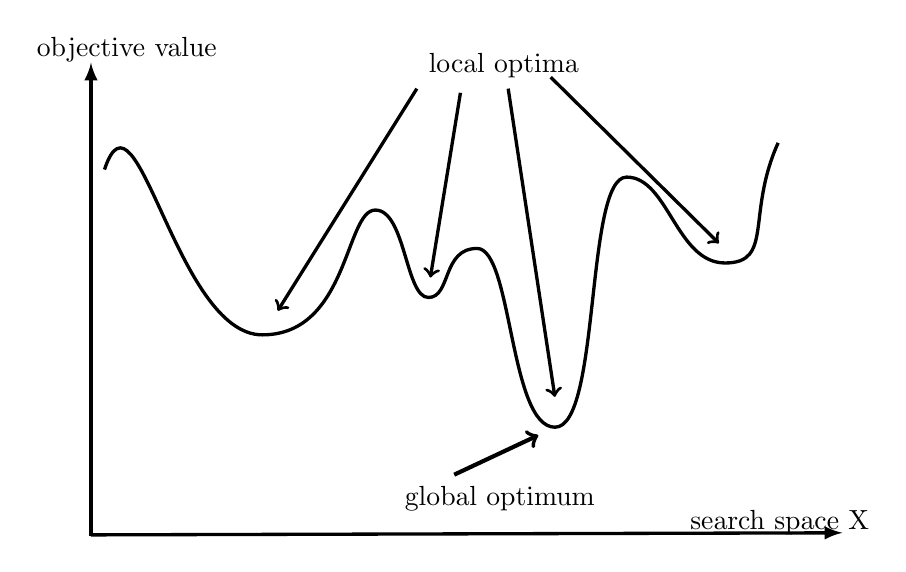
\begin{tikzpicture}[scale=0.5]
\pgftransformxscale{1.000000}
\pgftransformyscale{-1.000000}
\definecolor{dialinecolor}{rgb}{0.000000, 0.000000, 0.000000}
\pgfsetstrokecolor{dialinecolor}
\definecolor{dialinecolor}{rgb}{1.000000, 1.000000, 1.000000}
\pgfsetfillcolor{dialinecolor}
\pgfsetlinewidth{0.080000\du}
\pgfsetdash{}{0pt}
\pgfsetdash{}{0pt}
\pgfsetmiterjoin
\pgfsetbuttcap
{
\definecolor{dialinecolor}{rgb}{0.000000, 0.000000, 0.000000}
\pgfsetfillcolor{dialinecolor}
% was here!!!
\definecolor{dialinecolor}{rgb}{0.000000, 0.000000, 0.000000}
\pgfsetstrokecolor{dialinecolor}
\pgfpathmoveto{\pgfpoint{-12.454960\du}{6.637500\du}}
\pgfpathcurveto{\pgfpoint{-10.905125\du}{1.937500\du}}{\pgfpoint{-9.000000\du}{14.600000\du}}{\pgfpoint{-4.850000\du}{14.600000\du}}
\pgfpathcurveto{\pgfpoint{-0.700000\du}{14.600000\du}}{\pgfpoint{-0.854960\du}{8.587500\du}}{\pgfpoint{0.595040\du}{8.587500\du}}
\pgfpathcurveto{\pgfpoint{2.045040\du}{8.587500\du}}{\pgfpoint{2.050000\du}{12.800000\du}}{\pgfpoint{3.150000\du}{12.800000\du}}
\pgfpathcurveto{\pgfpoint{4.250000\du}{12.800000\du}}{\pgfpoint{3.800961\du}{10.437500\du}}{\pgfpoint{5.494875\du}{10.437500\du}}
\pgfpathcurveto{\pgfpoint{7.188790\du}{10.437500\du}}{\pgfpoint{7.050000\du}{19.050000\du}}{\pgfpoint{9.250000\du}{19.050000\du}}
\pgfpathcurveto{\pgfpoint{11.450000\du}{19.050000\du}}{\pgfpoint{10.700000\du}{7.000000\du}}{\pgfpoint{12.700000\du}{7.000000\du}}
\pgfpathcurveto{\pgfpoint{14.700000\du}{7.000000\du}}{\pgfpoint{15.095040\du}{11.137500\du}}{\pgfpoint{17.445040\du}{11.137500\du}}
\pgfpathcurveto{\pgfpoint{19.795040\du}{11.137500\du}}{\pgfpoint{18.450000\du}{8.800000\du}}{\pgfpoint{20.000000\du}{5.350000\du}}
\pgfusepath{stroke}
}
% setfont left to latex
\definecolor{dialinecolor}{rgb}{0.000000, 0.000000, 0.000000}
\pgfsetstrokecolor{dialinecolor}
\node[anchor=west] at (2.645040\du,1.637500\du){local optima};
% setfont left to latex
\definecolor{dialinecolor}{rgb}{0.000000, 0.000000, 0.000000}
\pgfsetstrokecolor{dialinecolor}
\node[anchor=west] at (5.095040\du,2.287500\du){};
% setfont left to latex
\definecolor{dialinecolor}{rgb}{0.000000, 0.000000, 0.000000}
\pgfsetstrokecolor{dialinecolor}
\node[anchor=west] at (1.495040\du,22.487500\du){global optimum};
\pgfsetlinewidth{0.080000\du}
\pgfsetdash{}{0pt}
\pgfsetdash{}{0pt}
\pgfsetbuttcap
{
\definecolor{dialinecolor}{rgb}{0.000000, 0.000000, 0.000000}
\pgfsetfillcolor{dialinecolor}
% was here!!!
\pgfsetarrowsend{to}
\definecolor{dialinecolor}{rgb}{0.000000, 0.000000, 0.000000}
\pgfsetstrokecolor{dialinecolor}
\draw (2.595040\du,2.737500\du)--(-4.104960\du,13.437500\du);
}
\pgfsetlinewidth{0.080000\du}
\pgfsetdash{}{0pt}
\pgfsetdash{}{0pt}
\pgfsetbuttcap
{
\definecolor{dialinecolor}{rgb}{0.000000, 0.000000, 0.000000}
\pgfsetfillcolor{dialinecolor}
% was here!!!
\pgfsetarrowsend{to}
\definecolor{dialinecolor}{rgb}{0.000000, 0.000000, 0.000000}
\pgfsetstrokecolor{dialinecolor}
\draw (4.695040\du,2.937500\du)--(3.245040\du,11.837500\du);
}
\pgfsetlinewidth{0.080000\du}
\pgfsetdash{}{0pt}
\pgfsetdash{}{0pt}
\pgfsetbuttcap
{
\definecolor{dialinecolor}{rgb}{0.000000, 0.000000, 0.000000}
\pgfsetfillcolor{dialinecolor}
% was here!!!
\pgfsetarrowsend{to}
\definecolor{dialinecolor}{rgb}{0.000000, 0.000000, 0.000000}
\pgfsetstrokecolor{dialinecolor}
\draw (6.995040\du,2.737500\du)--(9.245040\du,17.587500\du);
}
\pgfsetlinewidth{0.080000\du}
\pgfsetdash{}{0pt}
\pgfsetdash{}{0pt}
\pgfsetbuttcap
{
\definecolor{dialinecolor}{rgb}{0.000000, 0.000000, 0.000000}
\pgfsetfillcolor{dialinecolor}
% was here!!!
\pgfsetarrowsend{to}
\definecolor{dialinecolor}{rgb}{0.000000, 0.000000, 0.000000}
\pgfsetstrokecolor{dialinecolor}
\draw (9.045040\du,2.187500\du)--(17.145040\du,10.187500\du);
}
\pgfsetlinewidth{0.100000\du}
\pgfsetdash{}{0pt}
\pgfsetdash{}{0pt}
\pgfsetbuttcap
{
\definecolor{dialinecolor}{rgb}{0.000000, 0.000000, 0.000000}
\pgfsetfillcolor{dialinecolor}
% was here!!!
\pgfsetarrowsend{to}
\definecolor{dialinecolor}{rgb}{0.000000, 0.000000, 0.000000}
\pgfsetstrokecolor{dialinecolor}
\draw (4.395040\du,21.337500\du)--(8.445040\du,19.437500\du);
}
\pgfsetlinewidth{0.080000\du}
\pgfsetdash{}{0pt}
\pgfsetdash{}{0pt}
\pgfsetbuttcap
{
\definecolor{dialinecolor}{rgb}{0.000000, 0.000000, 0.000000}
\pgfsetfillcolor{dialinecolor}
% was here!!!
\pgfsetarrowsend{latex}
\definecolor{dialinecolor}{rgb}{0.000000, 0.000000, 0.000000}
\pgfsetstrokecolor{dialinecolor}
\draw (-13.104960\du,24.287500\du)--(-13.104960\du,1.487500\du);
}
\pgfsetlinewidth{0.080000\du}
\pgfsetdash{}{0pt}
\pgfsetdash{}{0pt}
\pgfsetbuttcap
{
\definecolor{dialinecolor}{rgb}{0.000000, 0.000000, 0.000000}
\pgfsetfillcolor{dialinecolor}
% was here!!!
\pgfsetarrowsend{latex}
\definecolor{dialinecolor}{rgb}{0.000000, 0.000000, 0.000000}
\pgfsetstrokecolor{dialinecolor}
\draw (-13.104960\du,24.237500\du)--(23.095040\du,24.137500\du);
}
% setfont left to latex
\definecolor{dialinecolor}{rgb}{0.000000, 0.000000, 0.000000}
\pgfsetstrokecolor{dialinecolor}
\node[anchor=west] at (15.245040\du,23.637500\du){search space X};
% setfont left to latex
\definecolor{dialinecolor}{rgb}{0.000000, 0.000000, 0.000000}
\pgfsetstrokecolor{dialinecolor}
\node[anchor=west] at (-16.235862\du,0.837500\du){objective value};
% setfont left to latex
\definecolor{dialinecolor}{rgb}{0.000000, 0.000000, 0.000000}
\pgfsetstrokecolor{dialinecolor}
\node[anchor=west] at (-16.235862\du,1.895833\du){};
\end{tikzpicture}
\caption{Local and global optima}
\end{figure}
\end{center}
\section{Tabu Search}
\label{sec:ts}
The Simple Tabu Search (TS) outlined in \ref{alg:ts}, chooses the best fitting solution out of the neighborhood $\mathcal{N}(s)$, which is not held in a short term memory, the so called tabu list. It holds recently visited solutions and is used to prevent cycles. Moreover, since the tabu list causes the algorithm to accept uphill moves, it can help to escape from local minima. Each chosen solution is added to the tabu list, which is of a specified size and therefore the algorithm has to remove solutions from it, which is usually done in a FIFO order. Most implementations of TS -- like the one implemented in this thesis -- do not store whole solutions, but solution attributes like moves or differences between solutions. The size of the list is a crucial parameter in TS and has to be chosen wisely, since if it is chosen too short the algorithm may stuck in cycles of higher order more likely and if it is chosen too long, the search space is restricted too much. The algorithm terminates if a specified termination criterion is met.\\
\begin{algorithm}[h]
\KwIn{A COP $P=(S,f)$}
\KwOut{A feasible Solution $s$}
$s \gets$ GenerateInitialSolution($S$)\;
$TabuList \gets \emptyset$
\While{NOT termination criterion}{
$s' \gets$ ChooseBestOf($\mathcal{N}(s) \setminus TabuList$)\;
Update($TabuList$)\;
}
\Return{$s$}
\caption{Tabu Search}
\label{alg:ts}
\end{algorithm}


\section{Integer Linear Programming}
Linear Programming (LP) or Mathematical Programming is an important field of operations research. Formulating a Linear Program (LP) is a mathematical way to define a COP and consists of defining the following inequations and equations: an objective function, a set of constraints on the variables $x$ and a set of constraints on their domain, which are all inequations.  All LPs can be written in the following form:

\begin{equation*}
\begin{aligned}
max. && c^Tx            \\
s.t. && Ax \leq b       \\
&& x \in \mathbb{R}^n \\
\end{aligned}
\end{equation*}

For each maximization problem there exists a minimization problem and vice versa, in the way that both problems are equivalent. The following set of equations defines the dual problem to the primal maximization problem:

\begin{equation*}
\begin{aligned}
min. && b^Ty            \\
s.t. && A^Ty \geq c       \\
&& y \in \mathbb{R}^n 	\\
\end{aligned}
\end{equation*}

Restrictions on the domain of the variables dedicates the LP into one of the following categories. Be $x$ the set of variables:
\begin{enumerate}
\item Linear Program (LP): $x \in \mathbb{R}^n$
\item Integer Linear Program (ILP): $x \in \mathbb{Z}^n$
\item Binary Integer Linear Program (BIP): $x \in \{0,1\}^n$
\item Mixed Integer Linear Program (MIP): variables can be restricted to different domains
\end{enumerate}

Optimizing the objective function with respect to the constraints means to solve the problem exactly and is in general $\mathcal{NP}$-hard. It has to be considered that classifying the problem into complexity classes only gives a worst case analysis of the running time any algorithm would require. State-of-the-art solvers like CPLEX \footnote{http://www-01.ibm.com/software/commerce/optimization/cplex-optimizer/}, GUROBI \footnote{http://www.gurobi.com/}, XPRESS \footnote{www.solver.com/xpress-solver-engine} use the simplex or the interior point algorithm combined with solution pruning methods as Branch and Bound or Branch and Cut, what makes them acquire relatively good average running times and makes LP a widely used method in operations research today. For example, for the TSP the optimal tour through 15112 Cities was calculated in 2001. \cite{applegate-01}
